% Project URL: https://www.overleaf.com/project/5ca355b5e166ef203a2098c1
\documentclass{article}
\usepackage[utf8]{inputenc}
\usepackage{listings}
\usepackage{algorithm}
\usepackage{algorithmic}
\usepackage[type=png]{animate}
\usepackage{graphicx}
\usepackage{wrapfig}
\usepackage{float}
\graphicspath{ {images02/} }
\usepackage{hyperref}
\hypersetup{
    colorlinks=true,
    linkcolor=blue,
    urlcolor=cyan
}

\title{\textbf{cse210 ass02}}
\author{Palash A. (\textit{e17cse069})}
\date{\textsc{16 April, 2019}}

\begin{document}

\maketitle

\section{Knuth Morris Pratt algorithm}
\href{https://rebrand.ly/kmp-pa5795}{Watch the video on YouTube} or scan the QR code below:
\begin{figure}[H]
    \centering
    
\includegraphics[width=0.25\textwidth]{kmp_qr.png}
    \label{fig:qr}
\end{figure}

\section{Greedy vs Dynamic}

\subsection{Greedy Algorithm}
Greedy programming is used in optimization problems following a simple, intuitive strategy. The problem is broken down into sub problems and the best solution at that step is chosen. Greedy algorithm may not give the optimal solution to every problem and in general is used if the following two conditions are met: \\
1. \textbf{Greedy Choice}: A global optimal solution can be obtained by choosing the optimal solution at each step. \\
2. \textbf{Optimal substructure}: The global optimal solution solution to the problem contains the optimal solutions to every sub problem.

\subsubsection{Example}
\textsc{Huffman Encoding} [\ref{sec:huffman}] is where the greedy approach is useful. Another algorithm that uses the greedy approach is \textsc{Djikstra's algorithm} to find the shortest path between two vertices.

\subsection{Dynamic Programming}
Dynamic programming is a problem solving approach where solutions to simpler, similar sub problems are stored to build the solution to a more complex problem. This bottom up approach is similar to recursion (where base cases allow us to determine final value) and works best when the new values are dependent on the previously calculated values. Dynamic programming has one condition that the problem must meet to be used that it should have overlapping sub problems. If not, divide and conquer may be used to solve the problem where memoization is not required increasing space efficiency of the solution.

\subsubsection{Example}
Dynamic Programming is exceptionally useful in solving problems such as \textsc{Backpack Problem} (\textit{Given a set of treasures with known values and weights, which ones should be picked to maximize profit within the capacity of the backpack}), \textsc{Longest Common Subsequence} (\textit{Given two sequences, which is the longest subsequence common to both}), and a better way to compute \textsc{Fibonacci Numbers} than recursion.

\subsection{Comparison}
The main difference between the two is the \textbf{greedy choice property}. Greedy programming chooses the most optimal solution based on the choices so far and not on future or all choices. Whereas, dynamic programming is exhaustive and is guaranteed to find the optimal solution. In other words, greedy algorithms do not reconsider choices.

For example, consider the following tree where the problem is to find the path with the max sum of node values.

\begin{figure}[H]
    \centering
    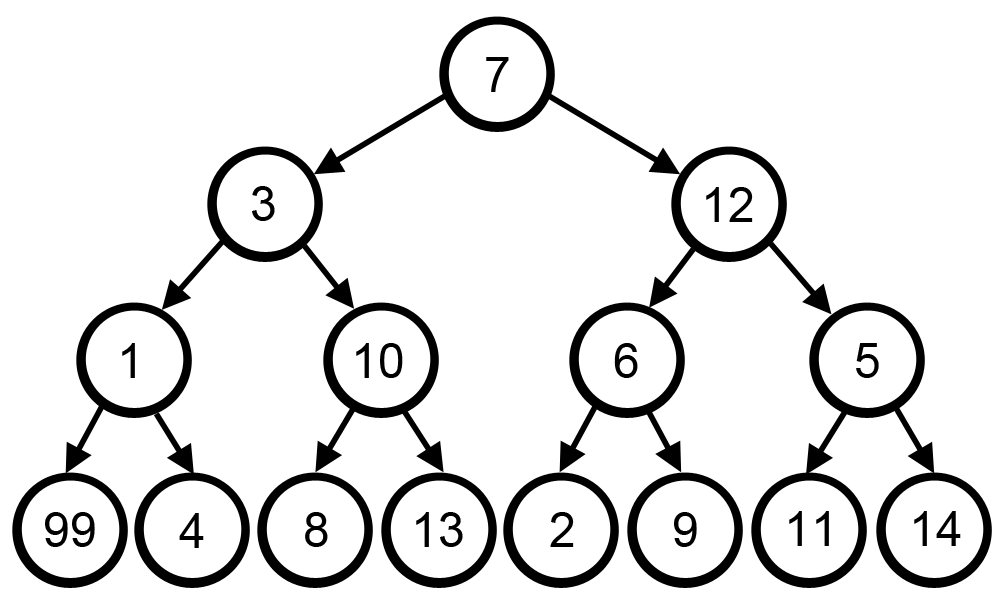
\includegraphics[width=0.75\textwidth]{greedy.png}
    \caption{Find the path with max sum}
    \label{fig:greedy}
\end{figure}
The path followed by the greedy approach is $7-12-6-9$ (by choosing the maximum value at each step).  However, using the DP approach, the tree problem can be broken down as such:\\
$solution = 7 + max(left\_subtree, right\_subtree)$, which can be further broken down for the respective subtrees until the leaf nodes are reached. On woking its way back up, this approach will follow the path $99-1-3-7$ yielding $110$ as the solution.

Hence, the path with the highest value is clearly $7-3-1-99$. The greedy approach fails in this problem to find the global optimal solution as it does not reconsider the choices and works from top down as compared to DP which solves the problem exhaustively and finds the optimal solution.

\section{Floyd Warshall Algorithm}
The Floyd Warshall algorithm is a shortest path algorithm for a graph that finds the shortest path (based on weights) between all pairs of vertices.
\subsection{Algorithm}
\begin{algorithm}
\label{algo:fwa}
\caption{Floyd Warshall Algorithm}
\begin{algorithmic}
\STATE $ V \leftarrow$ (number of vertices)
\STATE $dist \leftarrow |V|*|V|$
\FOR{v in V}
    \STATE $dist[v][v] \leftarrow 0$
\ENDFOR
\FOR{edge (u,v)}
    \STATE $dist[u][v] = weight(u,v)$
\ENDFOR
\FOR{k from 1 to V}
    \FOR{i from 1 to V}
        \FOR{j from 1 to V}
            \IF{$dist[i][j] > dist[i][k] + dist[k][j]$}
                \STATE $dist[i][j] \leftarrow dist[i][k] + dist[k][j]$
            \ENDIF
        \ENDFOR
    \ENDFOR
\ENDFOR
\end{algorithmic}
\end{algorithm}
\newpage
\subsection{Example}
Consider the graph on the side\\
\begin{wrapfigure}{r}{0.25\textwidth}
    \begin{center}
        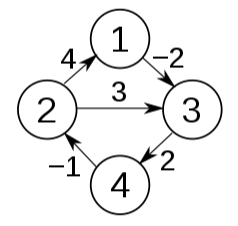
\includegraphics{fwa.png}
        \caption{Floyd Warshall Example Graph}
    \end{center}
    \label{fig:fwa}
\end{wrapfigure}
The following matrix is created after the first two for loops ($\infty$ is inserted where no path exists),\\
\begin{tabular}{|c||c|c|c|c|}
\hline
& 1 & 2 & 3 & 4 \\
\hline
\hline
1 & $0$ & $\infty$ & $-2$ & $\infty$ \\
\hline
2 & $4$ & $0$ & $3$ & $\infty$ \\
\hline
3 & $\infty$ & $\infty$ & $0$ & $2$ \\
\hline
4 & $\infty$ & $-1$ & $\infty$ & $0$ \\
\hline
\end{tabular}
\par
When $k=1$, the if condition fails for all values of $i$ and $j$ and hence, the table is unchanged.
\par
When $k=2$, the if condition passes when $(i=2,j=3)$ as $3 > 4 + (-2)$ and the matrix is updated as such,\\
\begin{tabular}{|c||c|c|c|c|}
\hline
& 1 & 2 & 3 & 4 \\
\hline
\hline
1 & $0$ & $\infty$ & $-2$ & $\infty$ \\
\hline
2 & $4$ & $0$ & \textit{2} & $\infty$ \\
\hline
3 & $\infty$ & $\infty$ & $0$ & $2$ \\
\hline
4 & $\infty$ & $-1$ & $\infty$ & $0$ \\
\hline
\end{tabular}
\\
The if condition also passes when $(i=4,j=1)$ and $(i=4,j=3)$ producing the following matrix:\\
\begin{tabular}{|c||c|c|c|c|}
\hline
& 1 & 2 & 3 & 4 \\
\hline
\hline
1 & $0$ & $\infty$ & $-2$ & $\infty$ \\
\hline
2 & $4$ & $0$ & $2$ & $\infty$ \\
\hline
3 & $\infty$ & $\infty$ & $0$ & $2$ \\
\hline
4 & \textit{3} & $-1$ & \textit{1} & $0$ \\
\hline
\end{tabular}
\par
When $k=3$, the if condition is passed when $(i=1,j=4)$ and when $(i=2,j=4)$ producing the following matrix:\\
\begin{tabular}{|c||c|c|c|c|}
\hline
& 1 & 2 & 3 & 4 \\
\hline
\hline
1 & $0$ & $\infty$ & $-2$ & \textit{0} \\
\hline
2 & $4$ & $0$ & $2$ & \textit{4} \\
\hline
3 & $\infty$ & $\infty$ & $0$ & $2$ \\
\hline
4 & $3$ & $-1$ & $1$ & $0$ \\
\hline
\end{tabular}
\par
When $k=4$, the if condition is passed when $(i=1,j=2)$, $(i=3,j=1)$, and $(i=3,j=2)$ producing the matrix:\\
\begin{tabular}{|c||c|c|c|c|}
\hline
& 1 & 2 & 3 & 4 \\
\hline
\hline
1 & $0$ & \textit{-1} & $-2$ & $0$ \\
\hline
2 & $4$ & $0$ & $2$ & $4$ \\
\hline
3 & \textit{5} & \textit{1} & $0$ & $2$ \\
\hline
4 & $3$ & $-1$ & $1$ & $0$ \\
\hline
\end{tabular}
\newpage
Hence, the shortest paths between all vertices in Figure \ref{fig:fwa} is given by the following matrix:
\begin{center}
    \begin{tabular}{|c||c|c|c|c|}
    \hline
    & 1 & 2 & 3 & 4 \\
    \hline
    \hline
    1 & $0$ & $-1$ & $-2$ & $0$ \\
    \hline
    2 & $4$ & $0$ & $2$ & $4$ \\
    \hline
    3 & $5$ & $1$ & $0$ & $2$ \\
    \hline
    4 & $3$ & $-1$ & $1$ & $0$ \\
    \hline
    \end{tabular}
\end{center}

\section{Huffman Encoding}
\label{sec:huffman}
Huffman encoding is an algorithm used for data compression and forms the basic idea behind file compression. Characters are stored using 8 bits. Huffman encoding reduces the size by encoding the most frequent characters with lesser bits, thereby reducing size. Huffman coding follows the \textsc{prefix rule} which states that no code is a prefix for another code.

Huffman coding works by building a binary tree of nodes based on character frequencies, where the lowest frequency is given the highest priority. The nodes in a Huffman tree are of two types - \textsc{Leaf nodes} which contain the character and the frequency of that character and \textsc{Internal nodes} which contain the total frequency till that node (counted from the leaf) and the links to the two child nodes. Priority queues are typically used to build the Huffman tree.

$0$ and $1$ is assigned to the left and right branch respectively and the codes are assigned to each character going from the root to the leaf. Hence, the most frequent characters will be encoded with the smallest codes, reducing size. [See example \ref{eg:huffman}]

\subsection{Algorithm}
\begin{algorithm}
\label{algo:huffman}
\caption{Huffman Tree Pseudocode}
\begin{algorithmic}
\REQUIRE A list $[C]$ of all characters with their frequencies
\STATE $n \leftarrow C.size$
\STATE $Q \leftarrow priority\_queue()$ \COMMENT {The priority is based on frequency, with lower frequency implying higher priority}
\FORALL{$c$ in $C$}
\item $Q.push(node(c))$
\ENDFOR
\WHILE{$Q.size() \neq 1$}
\STATE $i \leftarrow node()$
\item $i.left = Q.pop()$
\item $i.right = Q.pop()$
\item $i.frequency = i.left.frequency + i.right.frequency$
\item $Q.push(i)$
\ENDWHILE
\end{algorithmic}
\end{algorithm}

\subsection{Example}
\label{eg:huffman}
For example, consider a string of $100$ characters with the following character frequencies: \{$a:45$, $b:13$, $c:12$, $d:16$, $e:9$, $f:5$\}. Encoding the $100$ characters would require $100*8=800$ bits.
\begin{figure}[H]
    \centering
    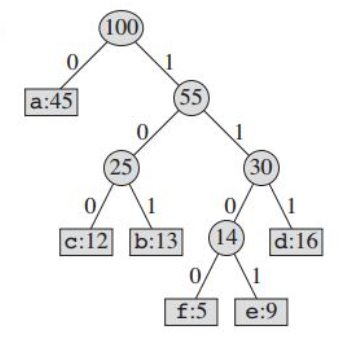
\includegraphics[width=0.5\textwidth]{huffman.png}
    \caption{Huffman Tree}
    \label{fig:huffman}
\end{figure}
The Huffman tree above produces the following codes:
\begin{center}
    \begin{tabular}{|c|c||c|c|}
        \hline
        Character & Frequency & Code & Bits needed \\
        \hline
        a & $45$ & \textsc{0} & $1*45=45$ \\
        b & $13$ & \textsc{101} & $3*13=39$ \\
        c & $12$ & \textsc{100} & $3*12=36$ \\
        d & $16$ & \textsc{111} & $3*16=48$ \\
        e & $9$ & \textsc{1101} & $4*9=36$ \\
        f & $5$ & \textsc{1100} & $4*5=20$ \\
        \hline
    \end{tabular}
    \\
    \textsc{Total bits needed}: $45+39+36+48+36+20=224$
\end{center}
Hence, Huffman encoding reduces the bits needed to represent the string from $800$ bits to $224$ bits!

\section{Topological Sort}
Topological sorting for a directed acyclic graph is a linear ordering of vertices such that for every edge $u-v$, $u$ comes before $v$. A certain directed acyclic graph may have multiple linear orderings based on the algorithm used to topologically sort the graph.
\subsection{Example}
\begin{center}
    \begin{figure}[H]
        \centering
        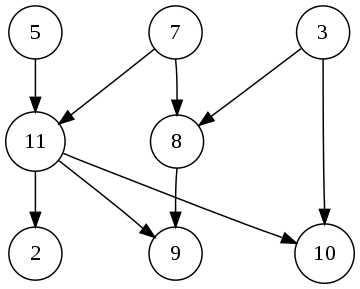
\includegraphics[width=0.5\textwidth]{dag.png}
        \caption{DAG for Topological Sort}
        \label{fig:dag}
    \end{figure}
\end{center}
The above graph can have multiple linear orderings based on different criteria:
\begin{itemize}
    \item \textsc{5, 7, 3, 11, 8, 2, 9, 10} 
    \textit{(visual: left-to-right, top-to-bottom)}
    \item \textsc{5, 7, 3, 8, 11, 10, 9, 2} 
    \textit{(fewest edges first)}
    \item \textsc{3, 5, 7, 8, 11, 2, 9, 10} 
    \textit{(smallest numbered vertex first)}
    \item \textsc{3, 7, 8, 5, 11, 10, 9, 2}
    \textit{(random)}
\end{itemize}
\subsection{Applications}
The main applications of this sort is to schedule jobs from the given jobs and their dependencies. In computer science, instruction scheduling, data serialization, and determining order of compilation (in case of makefiles) are some places where topological sorting is used.

\newpage
\section{Graph Search}
Breadth First Search and Depth First Search traversal order on the graph given below in Figure \ref{fig:graph}
\begin{figure}[H]
    \centering
    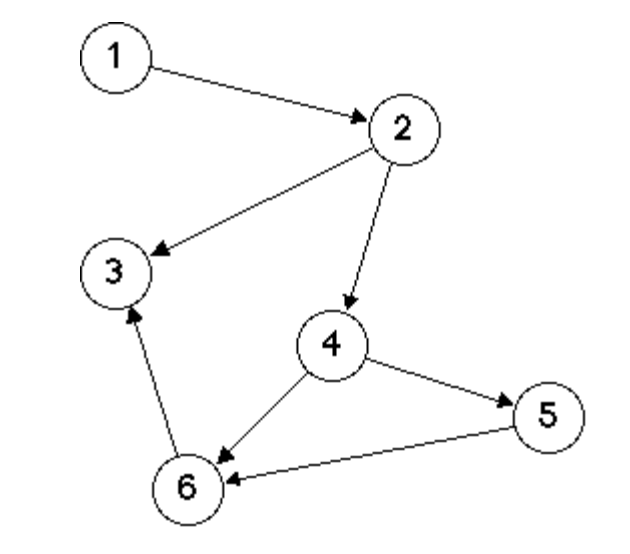
\includegraphics[width=0.5\textwidth]{images02/graph.png}
    \caption{Given graph}
    \label{fig:graph}
\end{figure}

\subsection{Breadth First Search}
\begin{center}
\begin{tabular}{ | c | c | } 
 \hline
 Nodes to visit & Nodes Visited \\
 \hline
 1 &  \\
 2 & 1 \\
 3,4 & 1,2 \\
 4 & 1,2,3 \\
 6,5 & 1,2,3,4 \\
 5 & 1,2,3,4,6 \\
  & 1,2,3,4,6,5 \\
 \hline
\end{tabular}
\end{center}
\begin{center}
Final order of traversal: [1,2,3,4,6,5]
\end{center}

\subsection{Depth First Search}
\begin{center}
\begin{tabular}{ | c | c | } 
 \hline
 Nodes to visit & Nodes Visited \\
 \hline
 1 &  \\
 2 & 1 \\
 3 & 1,2 \\
 4,6 & 1,2,3 \\
 6 & 1,2,3,4 \\
 5 & 1,2,3,4,6 \\
  & 1,2,3,4,6,5 \\
 \hline
\end{tabular}
\end{center}
\begin{center}
Final order of traversal: [1,2,3,4,6,5]
\end{center}

\end{document}